\subsection{Dataset Information}

The key characteristics of the MNIST dataset are summarized in \autoref{t:mnist}.

\begin{table}[H]
  \centering
  \begin{tblr}{
      hlines, vlines,
      cells = {c},
      column{1} = {l},
      cell{1}{1} = {c},
      row{1} = {bg=lightgray!100},
    }
    \textbf{Attribute}  & \textbf{Description} \\
    Number of Samples   & 70,000 \\
    Training Set        & 60,000 images \\
    Testing Set         & 10,000 images \\
    Image Size          & 28x28 pixels \\
    Channels            & 1 (grayscale) \\
    Classes             & 10 (digits 0-9) \\
  \end{tblr}
  \caption{MNIST Attributes}
  \label{t:mnist}
\end{table}

\subsection{Preprocessing}

To prepare the data for training, the following preprocessing steps were applied:

\begin{enumerate}
  \item 
    \textbf{Data Augmentation}: To increase the dataset size and improve model generalization, data augmentation 
    techniques were employed, including random rotations, shifts, and zooms.
  \item 
    \textbf{Reshaping}: Each image was reshaped to include a single channel (28x28x1) to conform to the input 
    requirements of the CNN.
  \item 
    \textbf{Normalization}: The pixel values of the images, initially ranging from 0 to 255, were scaled to a 
    range of 0 to 1 to improve the convergence of the model.
\end{enumerate}

\begin{minted}[
  frame=lines,
  baselinestretch=1.2,
  linenos
]
{python}
transform = transforms.Compose([
    transforms.RandomRotation(10),  # Rotation
    transforms.RandomAffine(0, shear=10),  # Shearing
    transforms.RandomAffine(0, translate=(0.1, 0.1)),  # Shifting up and down
    transforms.RandomResizedCrop(28, scale=(0.8, 1.0)),  # Zooming
    transforms.Resize((28, 28)),  # Rescale
    transforms.ToTensor(),
    transforms.Normalize((0.1307,), (0.3081,))  # Normalize with MNIST mean and std
])
\end{minted}

\subsection{Model Architecture}

\begin{itemize}
  \item \textbf{Input Layer}: Accepts input images of size 28x28x1.
  \item \textbf{Convolutional Layers}: Extract spatial features using filters with kernel sizes of 3x3.
    \begin{itemize}
      \item First convolutional layer: 16 filters.
      \item Second convolutional layer: 32 filters, ReLU activation.
    \end{itemize}
  \item 
    \textbf{Pooling Layer}: A max pooling operation with a 2x2 window is applied after each convolutional layer 
    to reduce spatial dimensions and computational complexity.
  \item 
    \textbf{Flatten Layer}: Converts the 2D feature maps into a 1D vector to feed into the fully connected layers.
  \item \textbf{Fully Connected Layers}
    \begin{itemize}
      \item First dense layer: 128 neurons with ReLU activation.
      \item 
        Output layer: 10 neurons (one for each digit class) with softmax activation for probability distribution.
    \end{itemize}
  \item 
    \textbf{Dropout Layer}: A dropout regularization layer with a rate of 0.8 is applied after the first dense 
    layer to prevent overfitting.
\end{itemize}


\begin{figure}[H]
  \begin{center}
    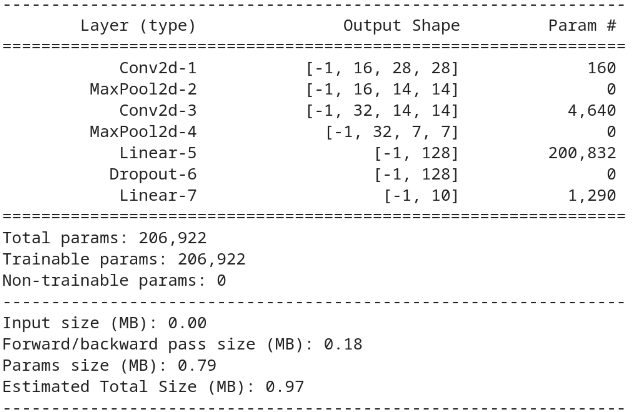
\includegraphics[width=0.7\textwidth]{img/methodology/model_summary.png}
    \caption{Model summary}
    \label{f:model_summary}
  \end{center}
\end{figure}

\autoref{f:model_summary} presents the output of the \texttt{summary} function from the Torchinfo package.

\subsection{Model Training}

The model was trained using the following configuration in \autoref{t:train_config}:

\begin{table}[H]
  \centering
  \begin{tblr}{
      hlines, vlines,
      cells = {c},
      column{1} = {l},
      cell{1}{1} = {c},
      row{1} = {bg=lightgray!100},
    }
    \textbf{Parameter}  & \textbf{Value} \\
    Loss Function       & Categorical cross-entropy \\
    Optimizer           & Adam optimizer with a learning rate of 0.001\\
    Batch Size          & 128 \\
    Number of Epochs    & 20 \\
  \end{tblr}
  \caption{Model Training Parameters}
  \label{t:train_config}
\end{table}
